%
% Main document
% ===========================================================================
% This is part of the document "Project documentation template".
% Authors: brd3, kaa1
%
%---------------------------------------------------------------------------
\documentclass[
	a4paper,					% paper format
	10pt,							% fontsize
	twoside,					% double-sided
	openright,				% begin new chapter on right side
	notitlepage,			% use no standard title page
	parskip=half,			% set paragraph skip to half of a line
]{scrreprt}					% KOMA-script report
%---------------------------------------------------------------------------

\raggedbottom
\KOMAoptions{cleardoublepage=plain}			% Add header and footer on blank pages


% Load Standard Packages:
%---------------------------------------------------------------------------
\usepackage[standard-baselineskips]{cmbright}

\usepackage[ngerman]{babel}										% german hyphenation
%\usepackage[latin1]{inputenc}  							% Unix/Linux - load extended character set (ISO 8859-1)
%\usepackage[ansinew]{inputenc}  							% Windows - load extended character set (ISO 8859-1)
\usepackage[T1]{fontenc}											% hyphenation of words with ä,ö and ü
\usepackage[utf8x]{inputenc}
\usepackage{textcomp}													% additional symbols
\usepackage{ae}																% better resolution of Type1-Fonts 
\usepackage{fancyhdr}													% simple manipulation of header and footer 
\usepackage{etoolbox}													% color manipulation of header and footer
\usepackage{graphicx}                      		% integration of images
\usepackage{float}														% floating objects
\usepackage{caption}													% for captions of figures and tables
\usepackage{booktabs}													% package for nicer tables
\usepackage{tocvsec2}													% provides means of controlling the sectional numbering
%---------------------------------------------------------------------------

% Load Math Packages
%---------------------------------------------------------------------------
\usepackage{amsmath}                    	   	% various features to facilitate writing math formulas
\usepackage{amsthm}                       	 	% enhanced version of latex's newtheorem
\usepackage{amsfonts}                      		% set of miscellaneous TeX fonts that augment the standard CM
\usepackage{amssymb}													% mathematical special characters
\usepackage{exscale}													% mathematical size corresponds to textsize
%---------------------------------------------------------------------------

% Package to facilitate placement of boxes at absolute positions
%---------------------------------------------------------------------------
\usepackage[absolute]{textpos}
\setlength{\TPHorizModule}{1mm}
\setlength{\TPVertModule}{1mm}
%---------------------------------------------------------------------------					
			
% Definition of Colors
%---------------------------------------------------------------------------
\RequirePackage{color}                          % Color (not xcolor!)
\definecolor{linkblue}{rgb}{0,0,0.8}            % Standard
\definecolor{darkblue}{rgb}{0,0.08,0.45}        % Dark blue
\definecolor{bfhgrey}{rgb}{0.41,0.49,0.57}      % BFH grey
%\definecolor{linkcolor}{rgb}{0,0,0.8}     			% Blue for the web- and cd-version!
\definecolor{linkcolor}{rgb}{0,0,0}        			% Black for the print-version!
%---------------------------------------------------------------------------

% Hyperref Package (Create links in a pdf)
%---------------------------------------------------------------------------
\usepackage[
	pdftex,ngerman,bookmarks,plainpages=false,pdfpagelabels,
	backref = {false},										% No index backreference
	colorlinks = {true},                  % Color links in a PDF
	hypertexnames = {true},               % no failures "same page(i)"
	bookmarksopen = {true},               % opens the bar on the left side
	bookmarksopenlevel = {0},             % depth of opened bookmarks
	pdftitle = {Template für Bachelor Thesis},	   	% PDF-property
	pdfauthor = {brd3},        					  % PDF-property
	pdfsubject = {LaTeX Template},        % PDF-property
	linkcolor = {linkcolor},              % Color of Links
	citecolor = {linkcolor},              % Color of Cite-Links
	urlcolor = {linkcolor},               % Color of URLs
]{hyperref}
%---------------------------------------------------------------------------
% Set up page dimension
%---------------------------------------------------------------------------
\usepackage{geometry}
\geometry{
	a4paper,
	left=28mm,
	right=15mm,
	top=30mm,
	headheight=20mm,
	headsep=10mm,
	textheight=242mm,
	footskip=15mm
}
%---------------------------------------------------------------------------

% Makeindex Package
%---------------------------------------------------------------------------
\usepackage{makeidx}                         		% To produce index
\makeindex                                    	% Index-Initialisation
%---------------------------------------------------------------------------

% Glossary Package
%---------------------------------------------------------------------------
% the glossaries package uses makeindex
% if you use TeXnicCenter do the following steps:
%  - Goto "Ausgabeprofile definieren" (ctrl + F7)
%  - Select the profile "LaTeX => PDF"
%  - Add in register "Nachbearbeitung" a new "Postprozessoren" point named Glossar
%  - Select makeindex.exe in the field "Anwendung" ( ..\MiKTeX x.x\miktex\bin\makeindex.exe )
%  - Add this [ -s "%tm.ist" -t "%tm.glg" -o "%tm.gls" "%tm.glo" ] in the field "Argumente"
%
% for futher informations go to http://ewus.de/tipp-1029.html
%---------------------------------------------------------------------------
\usepackage[nonumberlist]{glossaries}
\makeglossaries

% das zügs do unde dra find i eigendli unnötig, wenn mir so afön fülle mir sitewiss mit "`unüebliche"' begriffe! :(
\newglossaryentry{UML}{name={Wissensmodellierung},description={...}}
\newglossaryentry{Relationale Datenbank}{name={Beschreibungslogik },description={Reasoner ...}}
\newglossaryentry{Relationale Datenspeicherung}{name={Beschreibungslogik },description={Reasoner ...}}
\newglossaryentry{Semantische Datenbank}{name={Beschreibungslogik },description={Reasoner ...}}
\newglossaryentry{Expertensystem}{name={Beschreibungslogik },description={Reasoner ...}}
\newglossaryentry{Ontologie}{name={Ontologie},description={...}}
\newglossaryentry{Domäne}{name={Beschreibungslogik },description={Reasoner ...}}
\newglossaryentry{Wissensdomäne}{name={Beschreibungslogik },description={Reasoner ...}}
\newglossaryentry{Problemdomäne}{name={Beschreibungslogik },description={Reasoner ...}}
\newglossaryentry{Reasoner}{name={Beschreibungslogik },description={Reasoner ...}}
\newglossaryentry{Inferenzmaschine}{name={Beschreibungslogik },description={Reasoner ...}}
\newglossaryentry{Tutorial}{name={Beschreibungslogik },description={Reasoner ...}}
\newglossaryentry{RDF/XML}{name={Resolution},description={...}}
\newglossaryentry{OWL/XML}{name={Parser },description={...}}

\newglossaryentry{Semantik}{name={Inferenz},description={...}}
\newglossaryentry{Knowledge-Engineering}{name={Wissensmodellierung},description={...}}
\newglossaryentry{Knowledge-Engineer}{name={Wissensingeneur},description={Analytiker, Informationsmanager mit entsprechender Methodik und entsprechenden Werkzeugen}}
\newglossaryentry{HERMES}{name={Resolution},description={...}}
\newglossaryentry{Scrum}{name={Inferenz},description={...}}
\newglossaryentry{RDF}{name={Resolution},description={...}}
\newglossaryentry{OWL}{name={Inferenz},description={...}}
\newglossaryentry{Ontologie-Sprache}{name={Inferenz},description={...}}
\newglossaryentry{SWRL}{name={Inferenz},description={...}}
\newglossaryentry{SPARQL}{name={Inferenz},description={...}}
\newglossaryentry{W3C}{name={Inferenz},description={...}}
\newglossaryentry{Apache Stanbol}{name={Inferenz},description={...}}
\newglossaryentry{Stanford Protégé}{name={Inferenz},description={...}}
\newglossaryentry{Clark & Parsia Stardog}{name={Inferenz},description={...}}
\newglossaryentry{XML}{name={Inferenz},description={...}}
\newglossaryentry{Graphdatenbank}{name={Beschreibungslogik },description={Reasoner ...}}
\newglossaryentry{yWorks yEd}{name={Beschreibungslogik },description={Reasoner ...}}
\newglossaryentry{Unifikation}{name={Beschreibungslogik },description={Reasoner ...}}
\newglossaryentry{Semantisches Netz}{name={Parser },description={...}}
\newglossaryentry{NP-vollständig}{name={Parser },description={...}}
\newglossaryentry{URL}{name={Parser },description={...}}
\newglossaryentry{Turtle}{name={Parser },description={...}}
\newglossaryentry{FACT++}{name={Parser },description={...}}
\newglossaryentry{Pellet}{name={Beschreibungslogik },description={Reasoner ...}}
\newglossaryentry{SNARL}{name={Beschreibungslogik },description={Reasoner ...}}
%bis 6.2.1 ok
\newglossaryentry{Resolution}{name={Resolution},description={...}}
\newglossaryentry{Inferenz}{name={Inferenz},description={...}}

\newglossaryentry{Wissensakquise}{name={Wissensakquise},description={Sammeln/ erfassen, aufarbeiten/strukturieren von Wissen}}
\newglossaryentry{Parser}{name={Parser },description={...}}

\newglossaryentry{Beschreibungslogik}{name={Beschreibungslogik },description={Reasoner ...}}
\newglossaryentry{Frame}{name={Parser },description={...}}
\newglossaryentry{Wissensnetzte }{name={Parser },description={...}}

\newglossaryentry{Konzepte}{name={Parser },description={...}}
\newglossaryentry{Axiome}{name={Parser },description={...}}
\newglossaryentry{Prinzipien}{name={Parser },description={...}}
\newglossaryentry{Wissensmodellierung}{name={Beschreibungslogik },description={Reasoner ...}}

\newglossaryentry{Semantisches Web}{name={Beschreibungslogik },description={Reasoner ...}}
\newglossaryentry{Semantik}{name={Beschreibungslogik },description={Reasoner ...}}
\newglossaryentry{Formale Sprache}{name={Beschreibungslogik },description={Reasoner ...}}
\newglossaryentry{Künstliche Intelligenz}{name={Beschreibungslogik },description={Reasoner ...}}
\newglossaryentry{Aussagenlogik}{name={Beschreibungslogik },description={Reasoner ...}}
\newglossaryentry{Prädikatenlogik}{name={Beschreibungslogik },description={Reasoner ...}}

\newglossaryentry{Hierarchische Datenbank}{name={Beschreibungslogik },description={Reasoner ...}}
%\newglossaryentry{Graph}{name={Beschreibungslogik },description={Reasoner ...}}
%\newglossaryentry{Zyklenfreie Nachbarschaft}{name={Beschreibungslogik },description={Reasoner ...}}
%\newglossaryentry{Entität}{name={Beschreibungslogik },description={Reasoner ...}}
%\newglossaryentry{Knoten}{name={Beschreibungslogik },description={Reasoner ...}}
%\newglossaryentry{Kanten}{name={Beschreibungslogik },description={Reasoner ...}}
\newglossaryentry{Existenzaussage}{name={Beschreibungslogik },description={Reasoner ...}}
\newglossaryentry{Ontologiesprache}{name={Beschreibungslogik },description={Reasoner ...}}

\newglossaryentry{Modus Ponens}{name={Beschreibungslogik },description={Reasoner ...}}
\newglossaryentry{Theorem}{name={Beschreibungslogik },description={Reasoner ...}}

\newglossaryentry{Tableau-Kalkül}{name={Beschreibungslogik },description={Reasoner ...}}
\newglossaryentry{Prämisse}{name={Beschreibungslogik },description={Reasoner ...}}
\newglossaryentry{Konklusion}{name={Beschreibungslogik },description={Reasoner ...}}
\newglossaryentry{Literal}{name={Beschreibungslogik },description={Reasoner ...}}
\newglossaryentry{xxx}{name={Beschreibungslogik },description={Reasoner ...}}


%---------------------------------------------------------------------------

% Intro:
%---------------------------------------------------------------------------
\begin{document}                              	% Start Document
\settocdepth{section}														% Set depth of toc
\pagenumbering{roman}														
%---------------------------------------------------------------------------

\providecommand{\titel}{Titel des Berichts}		%  Hier den Titel des Berichts/Thesis eingeben					% Titel der Arbeit aus Datei titel.tex lesen
\providecommand{\versionnumber}{0.1}			%  Hier die aktuelle Versionsnummer eingeben
\providecommand{\versiondate}{08.06.2014}		%  Hier das Datum der aktuellen Version eingeben
				% Versionsnummer und -datum aus Datei version.tex lesen

% Set up header and footer
%---------------------------------------------------------------------------
\makeatletter
\patchcmd{\@fancyhead}{\rlap}{\color{bfhgrey}\rlap}{}{}		% new color of header
\patchcmd{\@fancyfoot}{\rlap}{\color{bfhgrey}\rlap}{}{}		% new color of footer
\makeatother

\fancyhf{}																		% clean all fields
\fancypagestyle{plain}{												% new definition of plain style	
	\fancyfoot[OR,EL]{\footnotesize \thepage} 	% footer right part --> page number
	\fancyfoot[OL,ER]{\footnotesize \titel, Version \versionnumber, \versiondate}	% footer even page left part 
}

\renewcommand{\chaptermark}[1]{\markboth{\thechapter.  #1}{}}
\renewcommand{\headrulewidth}{0pt}				% no header stripline
\renewcommand{\footrulewidth}{0pt} 				% no bottom stripline

\pagestyle{plain}
%---------------------------------------------------------------------------


% Title Page and Abstract
%---------------------------------------------------------------------------
%%
% Project documentation template
% ===========================================================================
% This is part of the document "Project documentation template".
% Authors: brd3, kaa1
%

\begin{titlepage}


% BFH-Logo absolute placed at (28,12) on A4 
% Actually not a realy satisfactory solution but working.
%---------------------------------------------------------------------------
\setlength{\unitlength}{1mm}
\begin{textblock}{20}[0,0](28,12)
	
\includegraphics[scale=1.0]{bilder/BFH_Logo_B.png}
\end{textblock}
\color{black}

% Institution / Titel / Untertitel / Autoren / Experten:
%---------------------------------------------------------------------------
\begin{flushleft}

\vspace*{21mm}

\fontsize{26pt}{40pt}\selectfont 
\titel 				\\							% Titel aus der Datei vorspann/titel.tex lesen
\vspace{2mm}

\fontsize{16pt}{24pt}\selectfont\vspace{0.3em}
Hier steht ein Untertitel 			\\							% Untertitel eingeben
\vspace{5mm}

\fontsize{10pt}{12pt}\selectfont
\textbf{Art der Arbeit (Semesterarbeit / Bachelorthesis / etc.)} \\									% eingeben
\vspace{7mm}

% Abstract (eingeben):
%---------------------------------------------------------------------------
\begin{textblock}{150}(28,100)
\fontsize{10pt}{12pt}\selectfont
[Kurztext (Abstract) einf�gen, falls gew�nscht] \\ 
Dieses Dokument dient als Vorlage f�r die Erstellung von Berichten nach den Richtlinien der BFH. Die Vorlage ist in \LaTeX{} erstellt und unterst�tzt das automatische Erstellen von diversen Verzeichnissen, Literaturangaben, Indexierung und Glossaren. Dieser kleine Text ist eine Zusammenfassung �ber das vorliegenden Dokument mit einer L�nge von 4 bis max. 8 Zeilen. \\
Das Titelbild kann in den Zeilen 157/158 der Datei template.tex ein- oder ausgeschaltet werden.
\end{textblock}

\begin{textblock}{150}(28,225)
\fontsize{10pt}{17pt}\selectfont
\begin{tabbing}
xxxxxxxxxxxxxxx\=xxxxxxxxxxxxxxxxxxxxxxxxxxxxxxxxxxxxxxxxxxxxxxx \kill
Studiengang:	\> [z.B. Elektro- und Kommunikationstechnik]	\\			% Namen eingeben
Autoren:		\> [Test Peter, M�ster R�s�]		\\					% Namen eingeben
Betreuer:	\> [Dr.~Xxxx Xxxx, Dr.~Yyyy Yyyy]		\\					% Namen eingeben
Auftraggeber:	\> [Wwwww AG]						\\					% Namen eingeben
Experten:		\> [Dr.~Zzzz Zzzz]				\\					% Namen eingeben
Datum:			\> \versiondate					\\		% aus Datei vorspann/version.tex lesen
\end{tabbing}

\end{textblock}
\end{flushleft}

\begin{textblock}{150}(28,280)
\noindent 
\color{bfhgrey}\fontsize{9pt}{10pt}\selectfont
Berner Fachhochschule | Haute �cole sp�cialis�e bernoise | Bern University of Applied Sciences
\color{black}\selectfont
\end{textblock}


\end{titlepage}

%
% ===========================================================================
% EOF
%
		% activate for Titelseite ohne Bild
%
% Project documentation template
% ===========================================================================
% This is part of the document "Project documentation template".
% Authors: brd3, kaa1
%

\begin{titlepage}


% BFH-Logo absolute placed at (28,12) on A4 and picture (16:9 or 15cm x 8.5cm)
% Actually not a realy satisfactory solution but working.
%---------------------------------------------------------------------------
\setlength{\unitlength}{1mm}
\begin{textblock}{20}[0,0](28,12)
    
\includegraphics[scale=1.0]{bilder/BFH_Logo_B.png}
\end{textblock}

\begin{textblock}{154}(28,48)
    \begin{picture}(150,2)
        \put(0,0){\color{bfhgrey}\rule{150mm}{2mm}}
    \end{picture}
\end{textblock}

\begin{textblock}{154}[0,-0.2](28,42)
    \centering
    
\includegraphics[scale=0.7]{bilder/owl.png}   % Titelbild definieren
\end{textblock}

\begin{textblock}{154} (28,135)
    \begin{picture}(150,2)
        \put(0,0){\color{bfhgrey}\rule{150mm}{2mm}}
    \end{picture}
\end{textblock}
\color{black}

% Institution / Titel / Untertitel / Autoren / Experten:
%---------------------------------------------------------------------------
\begin{flushleft}

\vspace*{120mm}

\fontsize{26pt}{28pt}\selectfont
\titel% Titel aus der Datei vorspann/titel.tex lesen
\vspace{3mm}



\fontsize{10pt}{12pt}\selectfont
\textbf{Aufbau von Wissensdomänen anhand einer semantischen Datenbank} \\                                 % eingeben
\vspace{3mm}

\begin{textblock}{150} (28,215)
\fontsize{10pt}{17pt}\selectfont
\begin{tabbing}
xxxxxxxxxxxxxxx\=xxxxxxxxxxxxxxxxxxxxxxxxxxxxxxxxxxxxxxxxxxxxxxx \kill
Autoren:        \> Sven Osterwalder, Mira Günzburger     \\                  % Namen eingeben
Datum:          \> \versiondate\\      % aus Datei vorspann/version.tex lesen
\end{tabbing}

\end{textblock}
\end{flushleft}

\begin{textblock}{150} (28,280)
\noindent 
\color{bfhgrey}\fontsize{9pt}{10pt}\selectfont
Berner Fachhochschule | Haute école spécialisée bernoise | Bern University of Applied Sciences
\color{black}\selectfont
\end{textblock}


\end{titlepage}

%
% ===========================================================================
% EOF
%
			% activate for Titelseite mit Bild
% Versionenkontrolle :
% -----------------------------------------------

\begin{textblock}{180} (15,150)
\color{black}
\begin{huge}
Versionen
\end{huge}
\vspace{10mm}

\fontsize{10pt}{18pt}\selectfont
\begin{tabbing}
xxxxxxxxxxx\=xxxxxxxxxxxxxxx\=xxxxxxxxxxxxxx\=xxxxxxxxxxxxxxxxxxxxxxxxxxxxxxxxxxxxxxxxxxxxxxx \kill
Version	\> Datum	\> Status		\> Bemerkungen		\\
0.1	\> 08.06.2014	\> Entwurf		\> Anforderungsdokument erstellen	\\	
0.2	\> 08.08.2014	\> Entwurf		\> Korrekturen und Ergänzungen	\\	
0.3	\> 19.09.2014	\> Entwurf		\> Anpassungen an die Aufgabenstellung	\\ 
%0.3	\> 02.09.2013	\> Entwurf		\> Donec eget aliquam urna. Lorem ipsum dolor sit amet	\\ 
%1.0	\> 12.09.2013	\> Definitiv	\> Lorem ipsum dolor sit ametPhasellus scelerisque, leo sed iaculis ornare 	\\ 
%1.1	\> 04.11.2013	\> Korrektur	\> Layout angepasst	\\
\end{tabbing}

\end{textblock}

\cleardoubleemptypage
\setcounter{page}{1}
\cleardoublepage
%\phantomsection 
%\addcontentsline{toc}{chapter}{Management Summary}
%\chapter*{Management Summary}
\label{chap:management_summary}

%\cleardoubleemptypage
%---------------------------------------------------------------------------

% Table of contents
%---------------------------------------------------------------------------
\tableofcontents
%\cleardoubleemptypage
%\cleardoublepage
%---------------------------------------------------------------------------

% Main part:
%---------------------------------------------------------------------------
\pagenumbering{arabic}
\chapter{Einleitung}
\label{chap:einleitung}

%CHeckliste fausibibel
%Ausgangslage, Problemstellung
%• Auftrag oder Aufgabenstellung
%• Resultat der Arbeit
%• Methodik (Herkunft der Daten, Vorgehen, Systemund
%Gültigkeitsgrenzen)
%• Folgerungen, offene Fragen

Der klassische Ansatz der Wissensabbildung, zum Beispiel in Form von UML, welchem die relationale Datenspeicherung zugrunde liegt, wird in der heutigen Informatik weitläufig eingesetzt und ist de facto Standard. Häufig geschieht dies in enger Verbindung mit der objektorientierten Programmierung. Experten aus einer Fachrichtung sind fähig diese Daten zu interpretieren und daraus Schlüsse zu ziehen. Es ist aber nicht möglich automatisch Fragestellungen zu beantworten, welche über reine Relationsverknüpfungen hinausgehen. Mit dieser Technik sind Objekteigenschaften und -Verhalten also eher schwer abbildbar. Eine andere Art Wissen zu repräsentieren sind semantische Datenbanken. Diese ermöglichen das Abbilden des Objektverhaltens und können mithilfe von Schlussfolgerungen die Rolle des Experten einnehmen.

In dieser Bachelorthesis soll eine solche semantische Datenbank aufgebaut und angewendet werden.  Die Arbeit wurde in zwei Teilen umgesetzt: Einem  theoretischen und einem praktischen Teil. Der theoretische Teil zeigt in Form eines Tutorials auf, wie ein knowledge engineer bei der Wissensmodellierung vorgeht. Er nutzt dabei Ontologien als Basis, um eine semantische Datenbank aufzubauen. Im praktischen Teil soll eine solche Ontologie aufgebaut und per Benutzerschnittstelle zugänglich gemacht werden.

Die gesteckten Ziele konnten allesamt erreicht werden. Es ist den Autoren gelungen die Theorie der Wissensmodellierung übersichtlich in einem Dokument aufzubereiten und wiederzugeben. Speziell dabei ist, dass in diesem fachliche Grundlagen mit einem praktischen Beispiel verbunden werden. Zusätzlich konnten auch konkrete Tipps aus der eigenen Erfahrung eingeflochten werden. Dieses Dokument ist dem Abschlussdokument als Anhang beigefügt.

Im praktischen Teil der Arbeit wurde ein Expertensystem für Reisen aufgebaut: ``In der heutigen Zeit werden Ferien häufig per Internet gebucht. Was aber, wenn der Urlaub nicht einfach zwei Wochen an einem Ort stattfinden soll? Was, wenn der Kunde reisen möchte? Oder sonstige spezielle Wünsche hat? Für solche Anforderungen muss er auch heute noch in ein Reisebüro um sich beraten zu lassen.''\\
Bei der Automatisierung dieses Prozesses kommt die Ontologie ins Spiel, welche mithilfe von Eigenschaften, Kriterien und Regeln die Problemdomäne abbildet. Durch die Verwendung eines Reasoners können verschiedene Reisevorschläge gemacht werden.\\
Um eine sehr individuelle Reiseplanung zu erreichen, musste zuerst eine Ontologie in Form von Klassen, Individuen, Relationen und Eigenschaften erstellt werden. Ohne klaren Rahmen würde eine Ontologie zu komplex und zu gross. Daher bauten die Autoren die Ontologie anhand exemplarischer Tages und Wochenendausflügen in der Schweiz auf.\\
Als Ergebnis können die Autoren eine semantischen Datenbank präsentieren. Dabei wird die von ihnen gewählte Problemdomäne in einem klar gesteckten Rahmen abgedeckt und die Mächtigkeit der Wissensmodellierung veranschaulicht. Die Schnittstelle für Benutzer wurde in Form eines Assistenten umgesetzt, welcher den Benutzer durch die Möglichkeiten führt und ihn bei der Planung seiner Reise unterstützt. Damit konnten die Autoren verhindern, dass Benutzer gezwungen sind, Abfragen in einer komplexen Abfragesprache zu formulieren.

Die Wissensmodellierung auf Basis von Ontolgien ist auf ihre Weise eine mächtiges Werkzeug um Informationen mit Semantik zu versehen. Trotzdem hat diese Art der Modellierung gewisse Einschränkungen, welche von anderen auf Logik basierenden Sprachen, wie zum Beispiel Prolog, abgedeckt werden. Im Laufe der Arbeit erkannten die Autoren, dass es noch Bedarf an Weiterentwicklung im Bezug auf die angebotenen Werkzeuge gibt. So musste eine Kombination von zwei Werkzeugen verwendet werden um sämtliche Anforderungen umzusetzen.

% Hier beschreiben Sie kurz das Thema der Arbeit, den Kontext sowie in knappen Worten das Ergebnis. Dieser Abschnitt gleicht einem Management Summary. Ziel dieses Kapitels ist, dem Leser die Entscheidungsgrundlage zu liefern, ob er die Arbeit lesen soll oder nicht.

% Einträge im Verzeichnis erscheinen lassen ohne hier eine Referenz einzufügen
%\nocite{kopka:band1}

\chapter{Technische Anforderungen}
\label{chap:technischeAnforderungen}

Bei den Recherchen der Projektarbeit hat sich die Erkenntnis ergeben, das eine erfolgreiche Verarbeitung von Anfragen die folgenden Komponenten benötigt:
\begin{itemize}
	\item Abbildung der Umwelt mittels Wissensdatenbank
	\item Definieren von Regeln zur Ableitung von Schlüssen mittels Logik
	\item Spracherkennung 
	\item Interne und Externe Schnittstellen zur Kommunikation
\end{itemize}

Die oben genannten Komponenten werden bereits im Ansatz durch die in der Projektarbeit evaluierte Lösung - Apache Stanbol - zur Verfügung gestellt. Allerdings hat sich gezeigt, dass diese grössere Erweiterungen benötigen um die gewünschten Ergebnisse zu liefern.

\section{Architektur}
\label{sec:architektur}
Um verschiedenen Teile zusammen zu nutzen, bietet Apache Stanbol eine frei konfigurierbare Verkettung dieser an. Dies geschieht mittels einer sogenannten Enhancement-Chain. Konkret heisst das, dass eine beliebige Eingabe dieser Kette übergeben werden kann, worauf dann die erste Softwarekomponente der Kette die Eingabe verarbeitet und das Resultat an die nächste Komponente weiterreicht. Diese Vorgang wird durch sämtliche Komponenten der Kette fortgeführt bis schlussendlich das Endresultat an die  anfragende Entität zurückgegeben wird.

Die Arbeit der Bachelorthesis besteht also darin, die Enhancement-Chain und die einzelnen Entitäten zu konfigurieren und zu erweitern.

%enhancementstructure.png/ https://stanbol.apache.org/docs/trunk/components/enhancer/enhancementstructure.png

\section{Abbildung der Umwelt mittels Wissensdatenbank}
\label{sec:architektur_wissensdatenbank}
\subsection{Objekte abbilden}
\label{sec:architektur_wissensdatenbank_Objekte}
Die Abbildung der Umwelt geschieht in Apache Stanbol mittels dem sogenannten Entity Hub.
Dieser stellt Informationen zu Entitäten und Objekten einer spezifischen Wissensdomäne zur Verfügung. Die konkrete Arbeit mit dem Entity Hub besteht also darin Objekte, der für die Arbeit gewählten Domäne, als Entitäten abzubilden.
\subsection{Definieren von Regeln zur Ableitung von Schlüssen mittels Logik}
\label{sec:architektur_regeln}
Um nun aus der Wissensdatenbank Schlüsse ziehen zu können, werden Regeln benötigt. Regeln werden verwendet um mittels Bedingungen auf weitere Eigenschaften schliessen zu können.
Apache Stanbol unterstützt auf Prädikatenlogik basierende Regeln, welche innerhalb der Rule Store Komponente als Rezepte gespeichert werden. Diese sind nichts anderes als eine Zusammenfassung von Regeln, welche eine ähnliche Objektkategorie betreffen.

\section{Spracherkennung}
\label{sec:architektur_spracherkennung}
Um einen Eingabesatz auszuwerten, muss dieser erst als solcher erkannt werden. Konkret müssen also, die einzelnen Wörter als Tokens identifiziert und einer Sprachkategorie zugeorndet werden. Dies geschieht mittels der Spracheerkennungskomponente OpenNLP (open natural language processing). Diese Spracherkennung wird für die Englische Sprache von Stanbol schon weitgehend angeboten. Nach unseren Erkenntinissen ist dies mit der Deutschen Sprache genau so möglich, jedoch nicht gegeben. Dies muss also noch erarbeitet werden. Nach ersten Recherchen wird dazu der Tokenizer sowie der Parser von OpenLNP verwendet.TODO (Link)

\section{Interne und Externe Schnittstellen zur Kommunikation}
 \label{sec:architektur_schnittstellen}
Um die oben genannten Komponenten ansprechen und nutzen zu können, sind Schnittstellen zur Kommunikation unumgänglich.

\subsection{Interne Kommunikation}
\label{sec:architektur_schnittstellen_intern}
Intern nutzt Apache Stanbol, wie bereits beschrieben, die sogenannte Enhancement Chain um von einem gegebenen Input, mittels verschiedenen Komponenten, zu einem Output zu gelangen. Die Enhancement Chain basiert gemäss [TODO:Link] auf einer Graph-Struktur, welche sie zur Kommunikation nutzt.

\subsection{Externe Kommunikation}
\label{sec:architektur_schnittstellen_extern}
Jede Komponente von Apache Stanbol, so z.B. auch die Enhancement Chain sowie deren Einzelkomponenten, verfügt über ein REST-Interface. Dies dient zur Kommunikation gegen aussen. Ein schematischer Ablauf der Kommunikation wird in Abbildung \ref{fig:kommunikationKomponenten} grob dargestellt.

\begin{figure}[H]
	\centering
		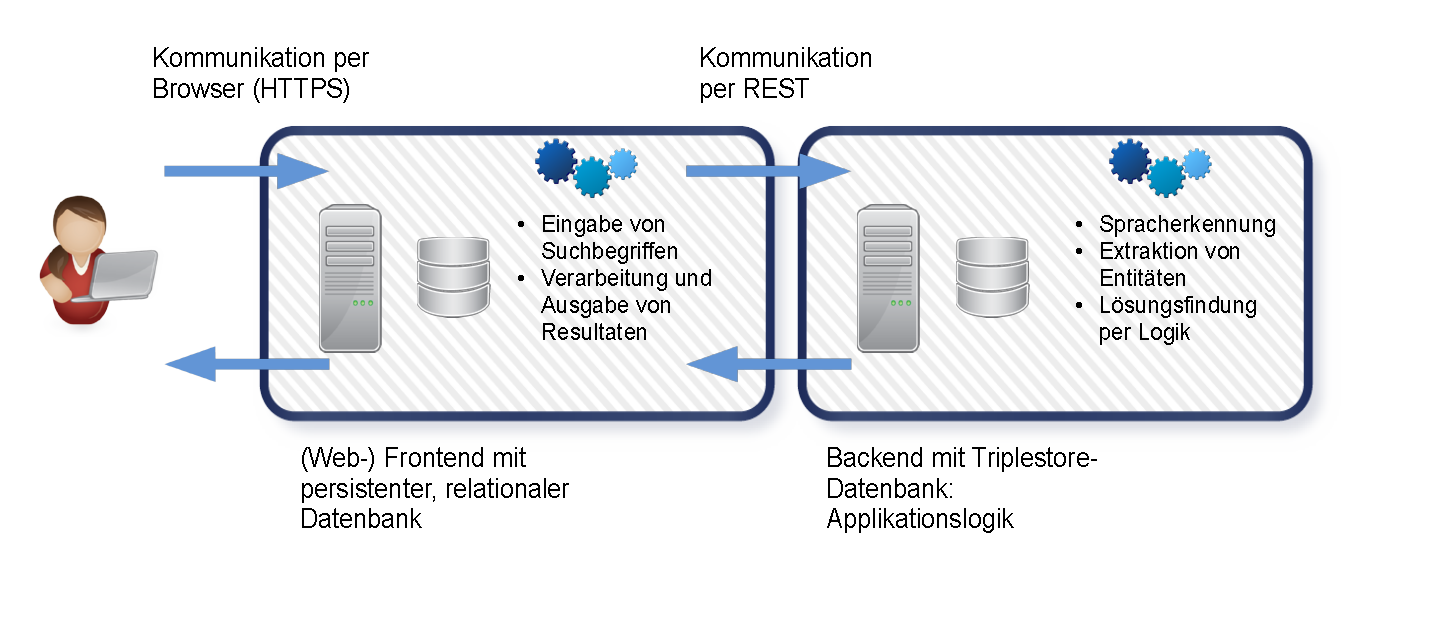
\includegraphics[scale=0.7]{bilder/software_komponenten.png}
	\caption{Kommunikation im Überblick}
	\label{fig:kommunikationKomponenten}
\end{figure}

\chapter{Wissensdomäne}
\label{chap:wissensdomäne}
Wie sich in der Vorarbeit herausgestellt hat, ist es notwendig die Domäne, in welcher Anfragen gestellt werden sollen, sehr detailliert abzubilden. Zudem ist die technische Umsetzung der Suche mittels Apache Stanbol weniger weit ausgearbeitet als ursprünglich angenommen. Um die Komplexität in einem angemessenen Rahmen zu halten, gilt es die Entitäten, also die Modellierung der Umwelt, stark einzuschränken. 
Als Folge dieser Erkenntnisse wird die Wissendomäne, mit welcher gearbeitet wird, eingeschränkt. Bei der gewählten Domäne handelt es sich um die Grundlagen der Programmierung am Beispiel der Programmiersprache Java.

\chapter{Ziel der Thesis}
\label{chap:thesisziel}
Als Endresultat der Thesis soll eine Applikation zur Verfügung stehen, welches es erlaubt eine Frage in deutscher Sprache zur Domäne der Programmierung anhand der Programmiersprache Java zu stellen. Dies kann dank der gegebenen REST-Schnittstelle z.B. direkt per Konsole oder aber per ansprechendem Web-Interface geschehen, welches aber nicht Teil der Thesis ist. Die Applikation soll in der Lage sein mittels der aufgebauten Wissensdatenbank, deren Relationen und schlussendlich Regeln die Frage zu beantworten. Kann eine Frage nicht eindeutig beantwortet werden, sollen zumindest Satzteile (Tokens) extrahiert und der entsprechende Inhalt zu diesen zurückgegeben werden. Eine Antwort ist dabei die Rückgabe einer Entität mit all deren Feldern, welchen dann von dem anfragenden Objekt entsprechend verarbeitet werden kann.

%---------------------------------------------------------------------------

% Glossary
%---------------------------------------------------------------------------
%\cleardoublepage
\phantomsection 
\addcontentsline{toc}{chapter}{Glossar}
\renewcommand{\glossaryname}{Glossar}
\printglossary
%---------------------------------------------------------------------------

% Bibliography
%---------------------------------------------------------------------------
%\cleardoublepage
\phantomsection 
\addcontentsline{toc}{chapter}{Literaturverzeichnis}
\bibliographystyle{IEEEtranS}
\bibliography{datenbanken/bibliography}{}
%---------------------------------------------------------------------------

% Listings
%---------------------------------------------------------------------------
%\cleardoublepage
\phantomsection 
\addcontentsline{toc}{chapter}{Abbildungsverzeichnis}
\listoffigures
%\cleardoublepage
\phantomsection 
\addcontentsline{toc}{chapter}{Tabellenverzeichnis}
\listoftables
%---------------------------------------------------------------------------

% Index
%---------------------------------------------------------------------------
%\cleardoublepage
\phantomsection 
\addcontentsline{toc}{chapter}{Stichwortverzeichnis}
\renewcommand{\indexname}{Stichwortverzeichnis}
\printindex
%---------------------------------------------------------------------------

% Attachment:
%---------------------------------------------------------------------------
\appendix
\settocdepth{section}
\chapter{Beliebiger Anhang}
\label{chap:bel_anhang}

Phasellus eget velit massa, sed faucibus nisi. Etiam tincidunt libero viverra lorem bibendum ut rutrum nisi volutpat. Donec non quam vitae lacus egestas suscipit at eu nisi. Maecenas non orci risus, at egestas tellus. Vivamus quis est pretium mauris fermentum consectetur. Cras non dolor vitae nulla molestie facilisis. Aliquam euismod nisl eget risus pretium non suscipit nulla feugiat. Nam in tortor sapien. Nam lectus nibh, laoreet eu ultrices nec, consequat nec sem. Nulla leo turpis, suscipit in vulputate a, dapibus molestie quam. Vestibulum pretium, purus sed suscipit tempus, turpis purus fermentum diam, id cursus enim mi a tortor. Proin imperdiet varius pellentesque. Nam congue, enim sit amet iaculis venenatis, dui neque ornare purus, laoreet porttitor nunc justo vel velit. Suspendisse potenti. Nulla facilisi.

\chapter{Weiterer Anhang}
\label{chap:anhang_B}

\section{Test 1}
Phasellus eget velit massa, sed faucibus nisi. Etiam tincidunt libero viverra lorem bibendum ut rutrum nisi volutpat. Donec non quam vitae lacus egestas suscipit at eu nisi. Maecenas non orci risus, at egestas tellus. Vivamus quis est pretium mauris fermentum consectetur. Cras non dolor vitae nulla molestie facilisis. Aliquam euismod nisl eget risus pretium non suscipit nulla feugiat. Nam in tortor sapien. 

\subsection{Umfeld}
Nam lectus nibh, laoreet eu ultrices nec, consequat nec sem. Nulla leo turpis, suscipit in vulputate a, dapibus molestie quam. Vestibulum pretium, purus sed suscipit tempus, turpis purus fermentum diam, id cursus enim mi a tortor. Proin imperdiet varius pellentesque. Nam congue, enim sit amet iaculis venenatis, dui neque ornare purus, laoreet porttitor nunc justo vel velit. Suspendisse potenti. Nulla facilisi.

\chapter{Inhalt der CD-ROM}
\label{chap:Inhalt_CDROM}

Inhaltsverzeichnis der beiliegenden CD-ROM, ev. Verzeichnisbaum, etc.
%---------------------------------------------------------------------------

%---------------------------------------------------------------------------
\end{document}

